\chapter{Summary and Outlook}\label{sec:zusammenfassung}

\section{Main Results}

This work connects arithmetic properties of a quadratic sequence with
classical geometry and shows how a simple Diophantine structure gives
rise to a three-dimensional helix. The principal results are:

\begin{enumerate}
\item Quadratic sequence


\[
k(n) = \frac{1}{6}(2n^2 + 3n + 1)
\]


with integer values precisely for


\[
n \equiv 1,5 \pmod{6}.
\]



\item Alternating step sizes (minor/major steps) with explicit formula


\[
a_k = \frac{1}{2}\bigl[(12k+3) + (-1)^{k+1}(4k+1)\bigr], \qquad k \geq 1.
\]



\item Circle circumferences


\[
U_m = 24m - 5
\]


with constant difference


\[
\Delta R = \frac{12}{\pi}.
\]



\item Archimedean spiral


\[
r(\theta) = \frac{6}{\pi^2}\theta.
\]



\item Simplified parametrisation via $p$:


\[
r(p) = \frac{6}{\pi\sqrt{3}}\sqrt{p},
\qquad
\theta(p) = \frac{\pi}{\sqrt{3}}\sqrt{p}.
\]



\item Exact arc-length integral


\[
L = \int_{p_1}^{p_2}
\frac{1}{\pi}\sqrt{\frac{3}{p} + \pi^2}\, dp.
\]



\item Taylor approximation with high accuracy:


\[
L \approx (p_2 - p_1)
+ \frac{3}{2\pi^2}\ln\!\left(\frac{p_2}{p_1}\right)
+ \frac{9}{8\pi^4}\left(\frac{1}{p_1} - \frac{1}{p_2}\right).
\]



\item Conical helix with half-angle


\[
\alpha = \arctan\!\left(\frac{2}{\pi}\right)
\approx 32.48^\circ.
\]



\item Integer points on the helix:


\[
\theta_n = \frac{\pi}{3}n + \frac{\pi}{4}.
\]



\item All primes $p>3$ appear as discrete points on the helix.
This follows as a corollary from the fact that all primes $p>3$
satisfy the congruence condition $p\equiv1,5\pmod{6}$ by a classical
result of number theory, and the helix is constructed so as to contain
all indices from these congruence classes. The helix additionally
contains all composite numbers with $n\equiv1,5\pmod{6}$; the primes
form a distinguished subset therein.
\end{enumerate}

\section{Methodological Significance}

This work demonstrates that arithmetic structures can not only be visualised
but \emph{geometrically forced}. The connection between:

\begin{itemize}
\item Number theory (congruences, prime numbers),
\item Analysis (integrals, Taylor series),
\item Geometry (spirals, cones, helices),
\item Classical constants ($\pi$, $\zeta(2)$)
\end{itemize}

leads to a surprisingly coherent three-dimensional structure.

The helix follows necessarily from:



\[
\Delta n = 6,
\qquad
\Delta r = \frac{12}{\pi},
\qquad
r \sim \sqrt{p},
\qquad
\theta \sim \sqrt{p}.
\]



\begin{figure}[htbp]
  \centering
  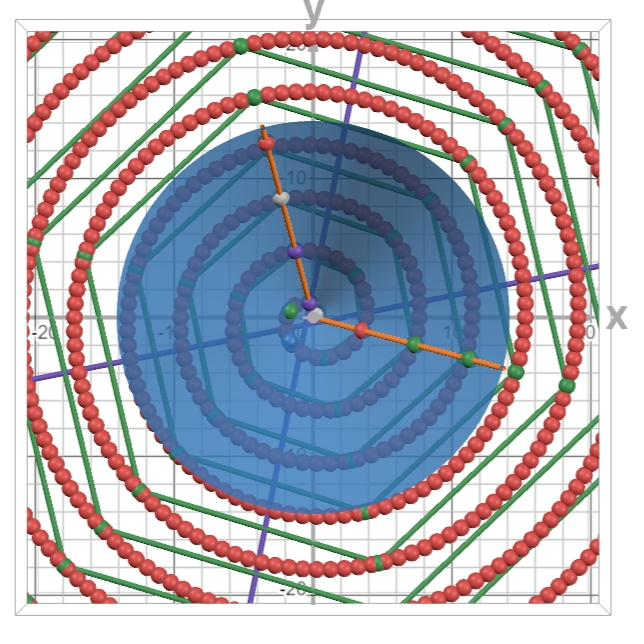
\includegraphics[width=0.72\textwidth]{bilder/spirale_topview}
  \caption{Top view of the conical helix (projection onto the $xy$-plane).
    The red spheres mark the equidistantly distributed points of the sequence
    on the spiral path. The green points (arranged hexagonally on six rays)
    show the function values $k(n)$ for all residue classes
    modulo~$6$; only the two rays with $n \equiv 1, 5 \pmod{6}$ yield
    integer values. The two diagonals run along these
    residue classes and make the $6$-periodicity of the arithmetic
    structure visually apparent. The blue disc shows the cone surface
    in projection; the spiral grows from inside to outside proportionally
    to $r \sim \theta$ (Archimedean).}
  \label{fig:spirale_topview}
\end{figure}

\section{Outlook}

The construction opens up several avenues for further investigation:

\begin{itemize}
\item \textbf{Prime gaps on the helix:}
  How do the distances between primes behave in the 3D model?

\item \textbf{Systematic comparison with the Ulam and Sacks spirals:}
  While the Ulam spiral~\cite{Stein1964} and the Sacks spiral~\cite{Sacks2003}
  are empirically motivated, the present construction possesses a closed-form
  derivation. A detailed comparison of the prime distributions
  across all three spiral types remains open.

\item \textbf{Distribution-theoretic refinements:}
  The spiral constant $a = 6/\pi^2$ coincides with the asymptotic mean
  of $\varphi(n)/n$ (Remark~\ref{rem:euler_coprimality}).
  Erd\H{o}s and Shapiro~\cite{ErdosShapiro1955} proved that the error
  term $H(x) = \sum_{n \leqslant x}\varphi(n)/n - 6x/\pi^2$ possesses
  a continuous distribution function; the Erd\H{o}s--Wintner
  theory~\cite{ErdosWintner1939} yields analogous results for
  $\varphi(n)/n$ itself. A natural follow-up question is whether the
  fluctuations of $\varphi(n)/n$ around the mean $6/\pi^2$ can be
  read off geometrically from the helix representation — for instance,
  as radial deviations of the integer-indexed points from the ideal
  spiral curve. Erd\H{o}s himself formulated the differentiability
  properties of this distribution function as an open
  problem~\cite{Erdos1974distribution}, which remains unsettled to
  this day.

\item \textbf{Zeros of $\zeta$ as arc lengths:}
  The arc-length parametrisation of Chapter~\ref{sec:parametrisierung}
  permits placing the imaginary parts $\gamma_n$ of the nontrivial
  zeros of $\zeta(s)$ on the spiral as marked points, with winding
  number $\theta(\gamma_n)/2\pi = \sqrt{\gamma_n/12}$. A numerical
  experiment with the first $200$ zeros shows their angular positions
  $\theta(\gamma_n) \bmod 2\pi$ to be equidistributed (Weyl sums at or
  below the $1/\sqrt{N}$ level; Kolmogorov--Smirnov statistic
  $D = 0.049$ against a $5\%$ critical value of $0.096$): with respect
  to this ruler the zeros behave angularly generically. Whether
  deviations from equidistribution appear at larger $N$, for the
  three-dimensional helix ruler, or for the zeros of $L(s,\chi_{-3})$
  in place of $\zeta$, is open.

\item \textbf{Generalisation to higher polynomial degrees:}
  Which geometries arise from cubic or quartic sequences?

\item \textbf{Modular interpretations:}
  Is there a connection to modular forms or lattice structures?

\item \textbf{Dynamical systems:}
  Can the helix be interpreted as the trajectory of a flow? In the
  elementary sense the answer is affirmative and explicit: in
  cylindrical coordinates the curve satisfies the autonomous system
  \[
    \dot r = a, \qquad \dot\varphi = 1, \qquad \dot z = c_1,
  \]
  with $\theta$ as time --- it is the trajectory of the constant
  vector field $(a,\, 1,\, c_1) = (6/\pi^2,\, 1,\, 3/\pi)$, and the
  position-independence of the winding distance~$d$ is the
  time-translation invariance of this flow. The integer points sample
  the trajectory at equal time steps $\Delta\theta = \pi/3$, six steps
  per revolution, so the residue classes modulo~$6$ appear as the six
  phases $\varphi \equiv (3+4r)\pi/12 \pmod{2\pi}$, $r = 0,\ldots,5$,
  of a stroboscopic (Poincar\'e) section; the integer-valued classes
  $n \equiv 1, 5 \pmod 6$ occupy the two fixed phases $7\pi/12$ and
  $23\pi/12$ --- the twin zones of Chapter~\ref{ch:helix}. The mod-$6$
  arithmetic of the sequence is thus the return-map bookkeeping of the
  flow. What remains open is the substantive part: this flow is linear
  and integrable, whereas a dynamics carrying arithmetic information
  in the sense of the spectral programme of
  Berry--Keating~\cite{BerryKeating1999} --- periodic orbits with
  periods $\ln p$, resonances at the zeros of $\zeta$ --- would have
  to be hyperbolic. Whether the cone can serve as the geometric
  carrier of such a dynamics is unknown.

\item \textbf{Asymptotic analysis:}
  The exact 3D curvature (Theorem~\ref{thm:3d-curvature-torsion}) and torsion
  are now known; their finer asymptotic analysis, particularly at
  the prime points, remains open.
\end{itemize}

This work shows that even simple sequences such as


\[
k(n) = \frac{2n^2 + 3n + 1}{6}
\]


give rise to a coherent geometric structure when consistently
transferred into three-dimensional space. The contribution of this work
is the synthesis: a single derivation path connecting known arithmetic
building blocks --- congruences, differences, circumference, cone, and
helix --- into one model.
